% ********************************** CHAPTER 1 source ***********************************************
\section{Struktura digitálního rádiového systému}



\marginpar{\textcolor{txt_blue}{Složení systému}} 
Tato práce se zabývá obecným digitálním rádiovým systémem. V leteckých aplikacích jsou rádiové systémy použity ve třech základních oblastech: komunikační, navigační a přehledové. Podle toho, jaký je primární účel systému, mění se i jeho složení a nastavení parametrů. Společná je jejich základní struktura: 

\begin{itemize}
\item Vysílač
\item Přenosový kanál
\item Přijímač
\end{itemize}

V dalším  budou analyzovány tyto tři komponenty oprostěné od funkcí specifických pro dané oblasti použití. To znamená, že nebude zahrnuto například různé kódování přenášené bitové posloupnosti (zdrojové či kanálové) a podobně. Vstupem vysílače je logický signál. Ten je modulován některou z mnoha digitálních modulací na nosný harmonický signál a anténou vyslán do prostoru. Přenosový kanál reprezentuje souhrnně vliv prostředí (přenosového média) na přenášený signál. Jako příklad je možno jmenovat: přidaný šum, útlum, vícecestné šíření, dopplerův posun, interference, omezení šířky pásma přenášeného signálu a jiné. Zkreslený signál je poté detekován a zpracován pomocí přijímače.


 
\vspace{0.25in}


%%%%%%%%%%%%%%%%%%%%%%%%%%%%%%%%%%%%%%% Popis vysílače %%%%%%%%%%%%%%%%%%%%%%

\subsection{Vysílač}

\marginpar{\textcolor{txt_blue}{Popis struktury vysílače}} 
Struktura vysílače, jak bude v následném textu chápána a analyzována je na obr. \ref{fig_block_Tx}. Vstupní signál $x_b(n)$ je bitovou posloupností nesoucí požadovanou informaci. Blok \textsl{Modulátor BB} přemění -- moduluje vstupní bitovou posloupnost na komplexní signál v základním pásmu (angl. \textsl{baseband}). Signál v základním pásmu $x_{rect}(t)$ pomocí aktuální úrovně své reálné a imaginární složky precizně definuje amplitudu a fázi nosné složky budoucího výstupního signálu vysílače  $x_{RF}(t)$. To je již signál s harmonickou nosnou, na kterou vybranou digitální modulací namodulována bitová posloupnost $x_b(n)$. 

\begin{figure}[ht]
 \begin{minipage}[c]{0.65\textwidth}
   
\tikzstyle{block} = [draw, fill=blue!20, rectangle, 
    minimum height=3em, minimum width=5em]
\tikzstyle{sum} = [draw, fill=blue!20, circle, node distance=1cm]
\tikzstyle{input} = [coordinate]
\tikzstyle{output} = [coordinate]
%\tikzstyle{pinstyle} = [pin edge={to-,thin,black}]

\begin{tikzpicture}[node distance=3cm,auto,>=latex']

    \node [input, name=input] {};
    \node [block, right of=input] (b_A) {Modulátor BB};
	\node [block, right of=b_A,xshift=2cm] (b_B) {Tvarování impulzu};
	\node [block, below of=b_B] (b_C) {Up-Convertor};
	\node [block, left of=b_C,xshift=-2cm] (b_D) {Přenosový kanál};
    \node [output, left of=b_D] (output) {};
 
    \draw [draw,->] (input) -- node {$x_b(n)$} (b_A);
	\draw [draw,->] (b_A) -- node {$x_{rect}(t)$} (b_B);
	\draw [draw,->] (b_B) -- node {$x_{rcos}(t)$} (b_C);
	\draw [draw,->] (b_C) -- node {$x_{RF}(t)$} (b_D);
    \draw [->] (b_D) -- node {$x_{dist}(t)$} (output);

\end{tikzpicture}

 \end{minipage}\hfill
 \begin{minipage}[t]{0.3\textwidth}
  \caption{Základní struktura digitálního rádiového vysílače.\label{fig_block_Tx}}
 \end{minipage}
\end{figure}

\marginpar{\textcolor{txt_blue}{Baseband modulace -- signál v základním pásmu}} 
 SDR (ať už simulované, nebo reálně využívané v této zprávě) používá k transformaci (konverzi) ze základního kmitočtového pásma do pásma nosného kmitočtu (angl. \textsl{passband}) obvod kmitočtové přeměny (tzv. směšovač) \textsl{Up-Convertor} typu kvadraturní modulátor. Tento typ obvodu vyžaduje komplexní vstupní signál v základním pásmu. Komplexní signál v základním pásmu je tvořen reálnou (soufázní, angl. \textsl{In-Phase}) a imaginární (kvadraturní, angl. \textsl{Quadrature}) složkou\footnote{Soufázní složka signálu bývá v technické praxi často označována jako signál I, kvadraturní pak jako Q.}. Blok \textsl{Modulátor BB} tvaruje ze vstupní posloupnosti $x_b(n)$ komplexní $x_{rect}r(t)$ signál, který je charakterizovaný svou tzv. bitovou (symbolovou) rychlostí (angl. \textsl{bitrate})\footnote{V případě \textsl{m-stavové} modulace je poměr bitové rychlosti k rychlosti symbolové dán počtem bitů přenesených v jednom symbolu.} a amplitudou. "\textsl{Modulátor BB}" je již navržen konkrétně pro daný typ výsledné digitální modulace signálu na výstupu vysílače $x_{RF}(t)$. Přicházející bity vstupní posloupnosti $x_b(n)$ jsou nejprve seskupovány podle typu výsledné modulace, viz.:

\begin{itemize}
\item dvoustavová: 1 symbol signálu $x_{rect}(t)$ odpovídá 1 bitu posloupnosti $x_b(n)$, 
\item čtyřstavová: 1 symbol signálu $x_{rect}(t)$ odpovídá 2 bitům posloupnosti $x_b(n)$,
\item osmistavová: 1 symbol signálu $x_{rect}(t)$ odpovídá 3 bitům posloupnosti $x_b(n)$, \ldots
\end{itemize}

Poté jsou seskupené bity tvořící \textsl{m-tice} (angl. \textsl{tuples}) mapovány na patřičnou reprezentaci pomocí komplexního signálu $x_{rect}(t)$. Pro každou kombinaci bitů symbolu je definována i kombinace úrovní\footnote{kvantizační úroveň může být dána přímo napětím, nebo vyjádřena jen číselně. To záleží na aktuální podobě obvodu Up-konvertoru. Někdy je vyžadován vstupní signál v základním pásmu, tzv. I a Q v analogové podobě. Moderní integrované obvody provádějící konverzi však často obsahují na vstupu dva DA převodníky a signál v základním pásmu je na ně přiváděn ve formě diskrétních I a Q vzorků.} soufázní a kvadraturní složky signálu $x_{rect}(t)$. Jedním ze základních parametrů digitálních rádiových systémů je i požadovaná přenosová \textsl{bitová} (angl. \textsl{bitrate}) a z ní odvozená \textsl{symbolová} (angl. \textsl{symbol--rate}) rychlost. Symbolová rychlost definuje dobu trvání jednoho symbolu (impulzu) $T_S$.

\begin{figure}[ht]
 \begin{minipage}[c]{0.65\textwidth}
  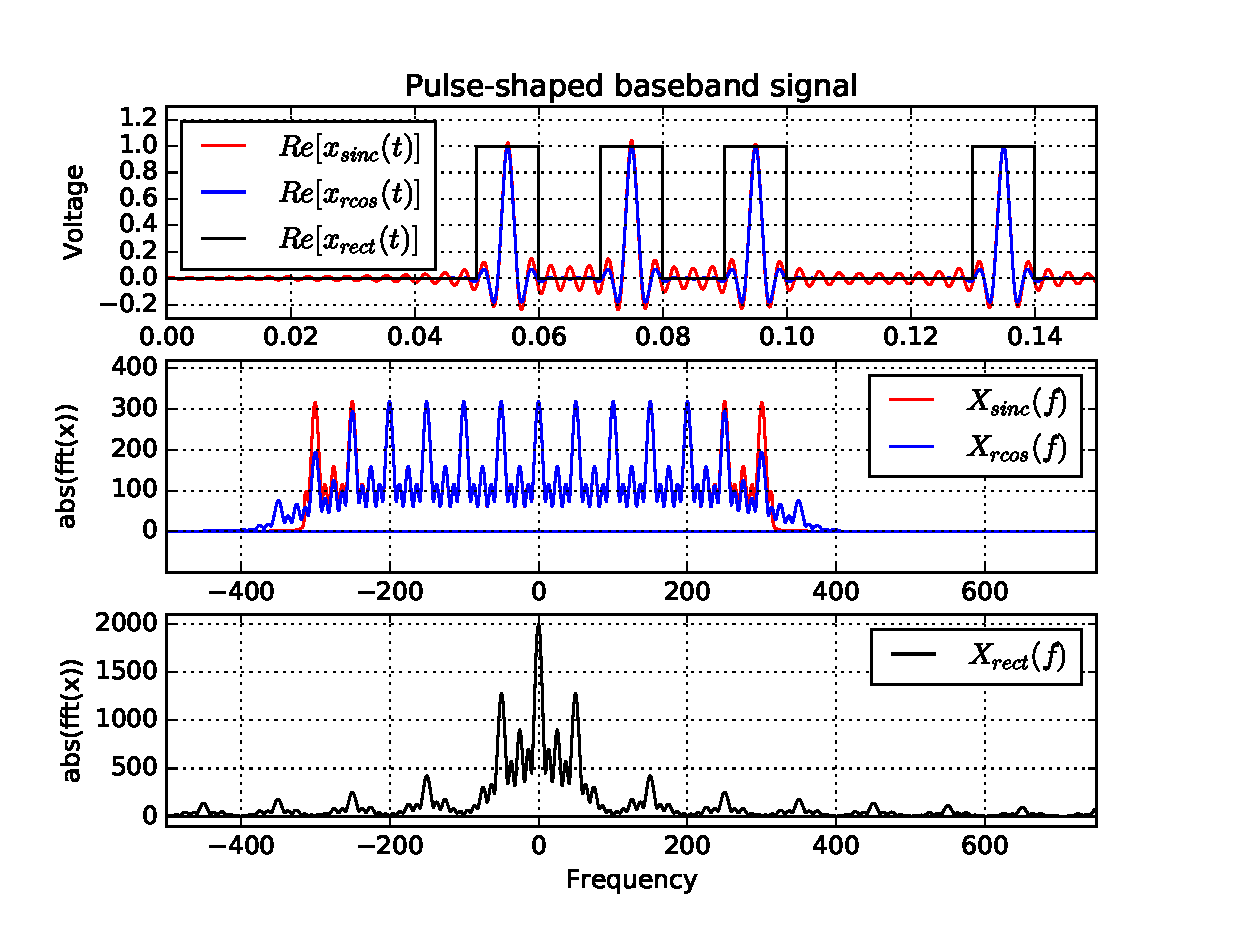
\includegraphics[width=4in]{./ch_02/img/Pulse_shaping.eps}
 \end{minipage}\hfill
 \begin{minipage}[t]{0.3\textwidth}
  \caption{Příklad tvarování impulzu signálu v základním pásmu. Kvůli jednoduchosti je znázorněná pouze jedna (uvažujme například, že reálná - symfázní) složka komplexního signálu.\label{fig_pulse_shaped}}
 \end{minipage}
\end{figure}

\marginpar{\textcolor{txt_blue}{Tvarování pulzu}}
Za blokem \textsl{Modulátoru BB} jsou přechody mezi jednotlivými symboly signálu $x_{rect}(t)$\footnote{U komplexního signálu v základním pásmu se už nehovoří o "bitech", ale o "symbolech". Přestože v tuto chvíli pojem "symbolu" ještě není precizně definován, je kvůli správnosti výkladu použit. Nicméně, v případě dvoustavových modulací obsahuje symbol jeden datový bit. Proto je možné setkat se někdy v technické literatuře s pojmem "bit" i v případě \textsl{baseband} signálu.} ideálně strmé, viz obr. \ref{fig_pulse_shaped}. Signál v základním pásmu (\textsl{baseband} signál) má v tuto chvíli podobu ideálních obdélníkových impulzů. Obdélníkový průběh je v reálných podmínkách nevýhodný. Skutečné přenosové kanály značně omezují kmitočtové spektrum přenášených signálů a potlačují některé kmitočty. Zjednodušeně lze jejich chování modelovat filtry typu dolní nebo pásmová propust\footnote{V angl. psané literatuře jsou označovány jako "\textsl{bandlimited channels}"}. Pro soudobé systémy pracující s vysokými bitovými (symbolovými) rychlostmi by nepredikovatelné zkreslení impulzu jednotlivých symbolů představovalo vážný problém při detekci a následném zpracování signálu v přijímači. Proto blok \textsl{Tvarování impulzu} kontrolovaně omezí pásmo signálu $x_{rect}(t)$ tím, že tvaruje jednotlivé impulzy symbolů podle vhodných matematických funkcí. Teoreticky je jich používáno více (\textsl{gauss}, \textsl{sinc}, \ldots), prakticky jsou používány funkce \textsl{raised-cosine} (ve zkratce \textsl{rcos}). V podstatě se jedná o "utlumenou" funkci sinc (angl. \textsl{damped sinc}). Výstupem bloku "\textsl{Tvarování impulzu}" je tedy signál $x_{rcos}(t)$, jehož kmitočtové spektrum je na rozdíl od signálu $x_{rect}(t)$ ohraničené a definované už v době návrhu systému. Signál $x_{rect}(t)$ s ideálně obdélníkovým průběhem, signál $x_{rcos}(t)$, kde je impulz tvarován funkcí raised-cosine a nakonec i signál $x_{sinc}(t)$ s impulzem ve tvaru funkce sinc spolu se svými kmitočtovými spektry jsou prezentovány na obrázku \ref{fig_pulse_shaped}. 



\marginpar{\textcolor{txt_blue}{Up-Convertor, Transformace do pásma VF}}
Komplexní signál $x_{rcos}(t)$ je připraven k transformaci (ke konverzi) do kmitočtového pásma vhodného pro daný systém. Většina SDR dnes využívá obvod \textsl{kvadraturní modulátor}. Tento typ modulátoru (často pojmenovávaného anglicky \textsl{Up-Convertor}) umožňuje obrovskou flexibilitu celého rádia. Je jedním z hlavních stavebních prvků SDR a příčinou "softwarového" přístupu k tvarování signálu rádia. Jde o to, že nezměněná hardwarová struktura může vygenerovat signál $x_{RF}(t)$ s takřka libovolnou digitální modulací. Záleží jen na tom, jak bude vypadat komplexní signál v základním pásmu $x_{rcos}(t)$. Ten, pomocí své reálné složky $Re[x_{rcos}(t)]$ a imaginární složky $Im[x_{rcos}(t)]$ přesně určuje fázi $\phi_{RF}(t)$ a amplitudu výsledného signálu $x_{RF}(t)$. Obrázek \ref{fig_quad_principle} demonstruje tento princip. Zde uvažujeme pouze digitální modulace s konstantní amplitudou nosného signálu. U nich je manipulováno jen s fází $\phi_{RF}(t)$\footnote{Skupina modulací manipulujících s fází (v angl. \textsl{PSK}, čili \textsl{phase shift keying})} nosného harmonického signálu.
 
\begin{figure}[ht]
 \begin{minipage}[c]{0.65\textwidth}
  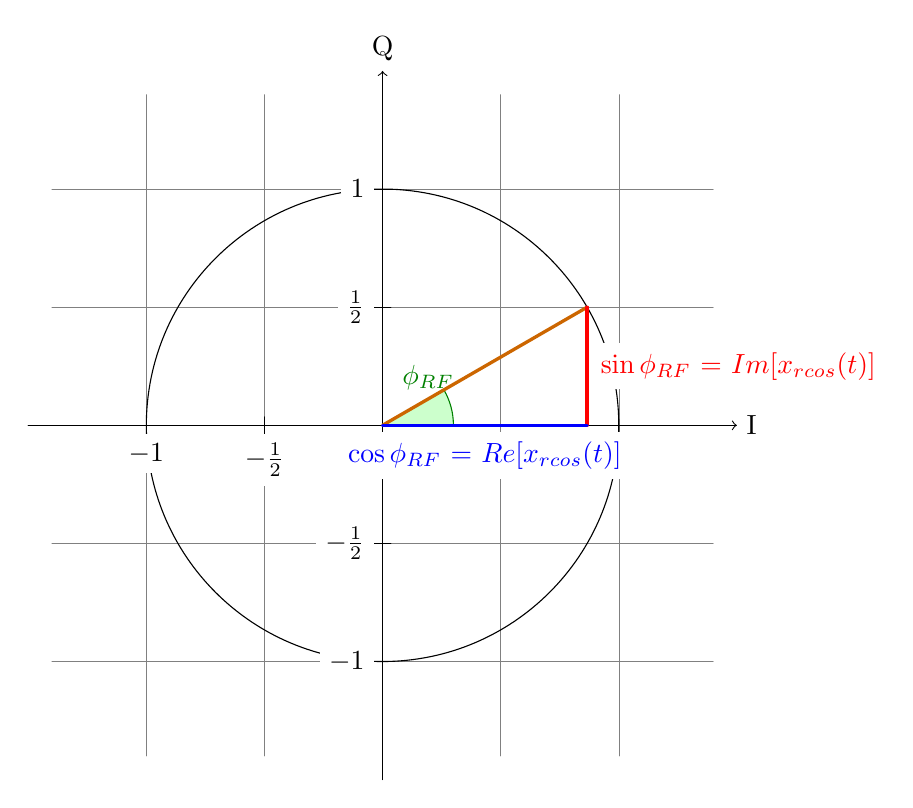
\begin{tikzpicture}[scale=3,cap=round]
  % Local definitions
  \def\costhirty{0.8660256}

  % Colors
  \colorlet{anglecolor}{green!50!black}
  \colorlet{sincolor}{red}
  \colorlet{amplcolor}{orange!80!black}
  \colorlet{coscolor}{blue}

  % Styles
  \tikzstyle{axes}=[]
  \tikzstyle{important line}=[very thick]
  \tikzstyle{information text}=[rounded corners,fill=red!10,inner sep=1ex]

  % The graphic
  \draw[style=help lines,step=0.5cm] (-1.4,-1.4) grid (1.4,1.4);

  \draw (0,0) circle (1cm);

  \begin{scope}[style=axes]
    \draw[->] (-1.5,0) -- (1.5,0) node[right] {I};
    \draw[->] (0,-1.5) -- (0,1.5) node[above] {Q};

    \foreach \x/\xtext in {-1, -.5/-\frac{1}{2}, 1}
      \draw[xshift=\x cm] (0pt,1pt) -- (0pt,-1pt) node[below,fill=white]
            {$\xtext$};

    \foreach \y/\ytext in {-1, -.5/-\frac{1}{2}, .5/\frac{1}{2}, 1}
      \draw[yshift=\y cm] (1pt,0pt) -- (-1pt,0pt) node[left,fill=white]
            {$\ytext$};
  \end{scope}

  \filldraw[fill=green!20,draw=anglecolor] (0,0) -- (3mm,0pt) arc(0:30:3mm);
  \draw (15:2mm) node[above=5pt,anglecolor] {$\phi_{RF}$};
  
  \draw [style=important line,amplcolor]
	(0,0) -- (30:1cm);

  \draw[style=important line,sincolor]
    (30:1cm) -- node[right=1pt,fill=white] {$\sin \phi_{RF}$ = $Im[x_{rcos}(t)]$} +(0,-.5);

  \draw[style=important line,coscolor]
    (0,0) -- node[below=2pt,fill=white] {$\cos \phi_{RF}$ = $Re[x_{rcos}(t)]$} (\costhirty,0);

 
\end{tikzpicture}

 \end{minipage}\hfill
 \begin{minipage}[t]{0.3\textwidth}
  \caption{Princip kvadraturní modulace. Význam symfázní a kvadraturní složky signálu základního pásma.\label{fig_quad_principle}}
 \end{minipage}
\end{figure}


Díky nízkým kmitočtům signálů základního pásma je možné k jejich tvarování využít procesorů (často obsahujících podpůrné struktury pro číslicové zpracování signálů) a tím pádem lze jejich strukturu i parametry určovat softwarem v procesoru. Přeneseně tedy software procesoru tvaruje (definuje) vysokofrekvenční signál na výstupu vysílače $x_{RF}(t)$.



